\section{北京理工大学本科生毕业设计论文模板使用指南}

\tipbox{注意:目前版本的毕业设计论文是按照北京理工大学计算机学院 2015 级毕业论文模板进行的设计与排版,如果 2016 级毕业论文模板有任何格式更新,我们会及时在这里更新。}

\subsection{熟悉项目}

\dirtree{%
  .1 /.
  .2 README.md.
  .2 main.tex.
  .2 main.pdf.
  .2 chapters.
  .3 0\_abstract.tex.
  .3 1\_chapter1.tex.
  .2 images.
  .3 bit\_logo.png.
  .3 header.png.
  .2 misc.
  .3 0\_cover.tex.
  .3 1\_originality.tex.
  .3 2\_toc.tex.
  .3 3\_conclusion.tex.
  .3 4\_reference.tex.
  .3 5\_appendix.tex.
  .3 6\_acknowledgements.tex.
  .3 ref.bib.
}

本项目由一个主文件和与之并存的几个辅助文件夹中的文件构成:

\begin{itemize}
  \item[\color{RubineRed}\textbf{\texttt{main.tex}}] 毕业论文模板的主文件
  \item[\color{RubineRed}\textbf{\texttt{./chapters}}] 文件夹:包含有整个毕业论文的“摘要”和正文的全部“章节”
  \begin{itemize}
    \item[\color{RoyalBlue}\texttt{0\_abstract.tex}] 毕业论文的“摘要”(中文摘要与英文摘要)
    \item[\color{RoyalBlue}\texttt{1\_chapter1.tex}] 毕业论文正文“第一章”(示例章节)
    \item[\color{RoyalBlue}\texttt{...}] (你可以继续添加第二章 \texttt{2\_chapter2.tex}、第三章 \texttt{3\_chapter3.tex}……,并在主文件 \texttt{main.tex} 中引用(详见下文)
  \end{itemize}
  \item[\color{RubineRed}\textbf{\texttt{./misc}}] 文件夹:包含有毕业论文模板中的封面、后置章节与参考文献
  \begin{itemize}
    \item[\color{RoyalBlue}\textbf{\texttt{0\_cover.tex}}] 毕业论文的“封面”,一般情况无需更改
    \item[\color{RoyalBlue}\textbf{\texttt{1\_originality.tex}}] 毕业论文的“原创性声明”,一般情况无需更改(签字和日期后期手动添加)
    \item[\color{RoyalBlue}\textbf{\texttt{2\_toc.tex}}] 毕业论文的“目录”,一般情况无需更改(由 {\LaTeX} 自动生成)
    \item[\color{RoyalBlue}\textbf{\texttt{3\_conclusion.tex}}] 毕业论文的“结论”,按照一般章节文件对待
    \item[\color{RoyalBlue}\textbf{\texttt{4\_reference.tex}}] 毕业论文的“参考文献”,一般情况无需更改(由 {\LaTeX} 根据你文档中的 \verb|\cite{}| 自动生成)
    \item[\color{RoyalBlue}\textbf{\texttt{5\_appendix.tex}}] 毕业论文的“附录”,按照一般章节文件对待
    \item[\color{RoyalBlue}\textbf{\texttt{6\_acknow...ments.tex}}] 毕业论文的“致谢”,按照一般章节文件对待
    \item[\color{RoyalBlue}\textbf{\texttt{ref.bib}}] 参考文献 \hologo{BibTeX} 数据库
  \end{itemize}
\end{itemize}

主文件与其余文件之间的引用关系大致如下图 \ref{grad_thesis_main_submodule} 所示:

\begin{figure}[H]
  \center
  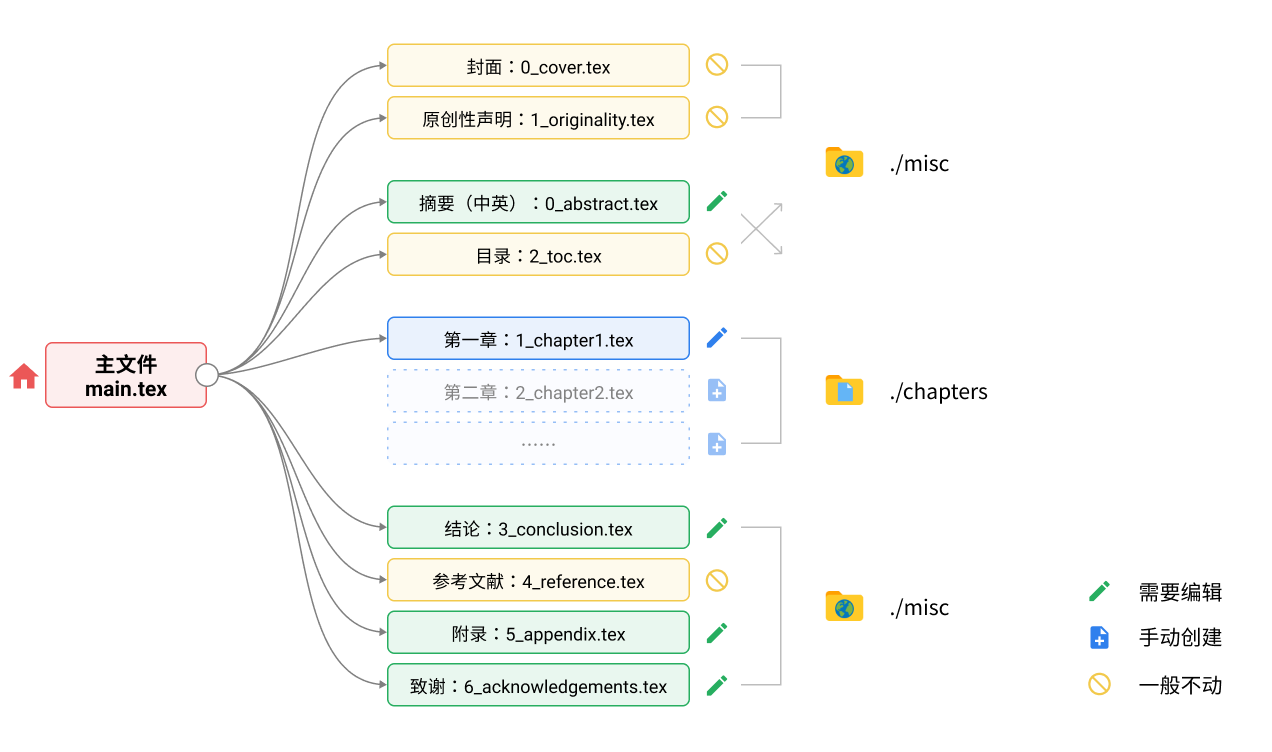
\includegraphics[width=\textwidth]{images/grad_thesis.png}
  \caption{毕业论文模板主模块与各个分支之间的关系}
  \label{grad_thesis_main_submodule}
\end{figure}

具体编译和使用,请见下文详细描述。

\subsection{使用与编译方式}

\subsubsection{使用 Overleaf 直接打开}

本模板已经发布在 Overleaf 上,你可以打开直接使用:

\begin{center}
  \color{ForestGreen}\href{https://www.overleaf.com/latex/templates/bei-jing-li-gong-da-xue-ben-ke-sheng-bi-ye-she-ji-lun-wen-mo-ban/mwhjgqsncxxg}{https://www.overleaf.com/latex/templates/bei-jing-li-gong-da-xue-ben-ke-sheng-bi-ye-she-ji-lun-wen-mo-ban/mwhjgqsncxxg}
\end{center}

\begin{figure}[H]
  \centering
  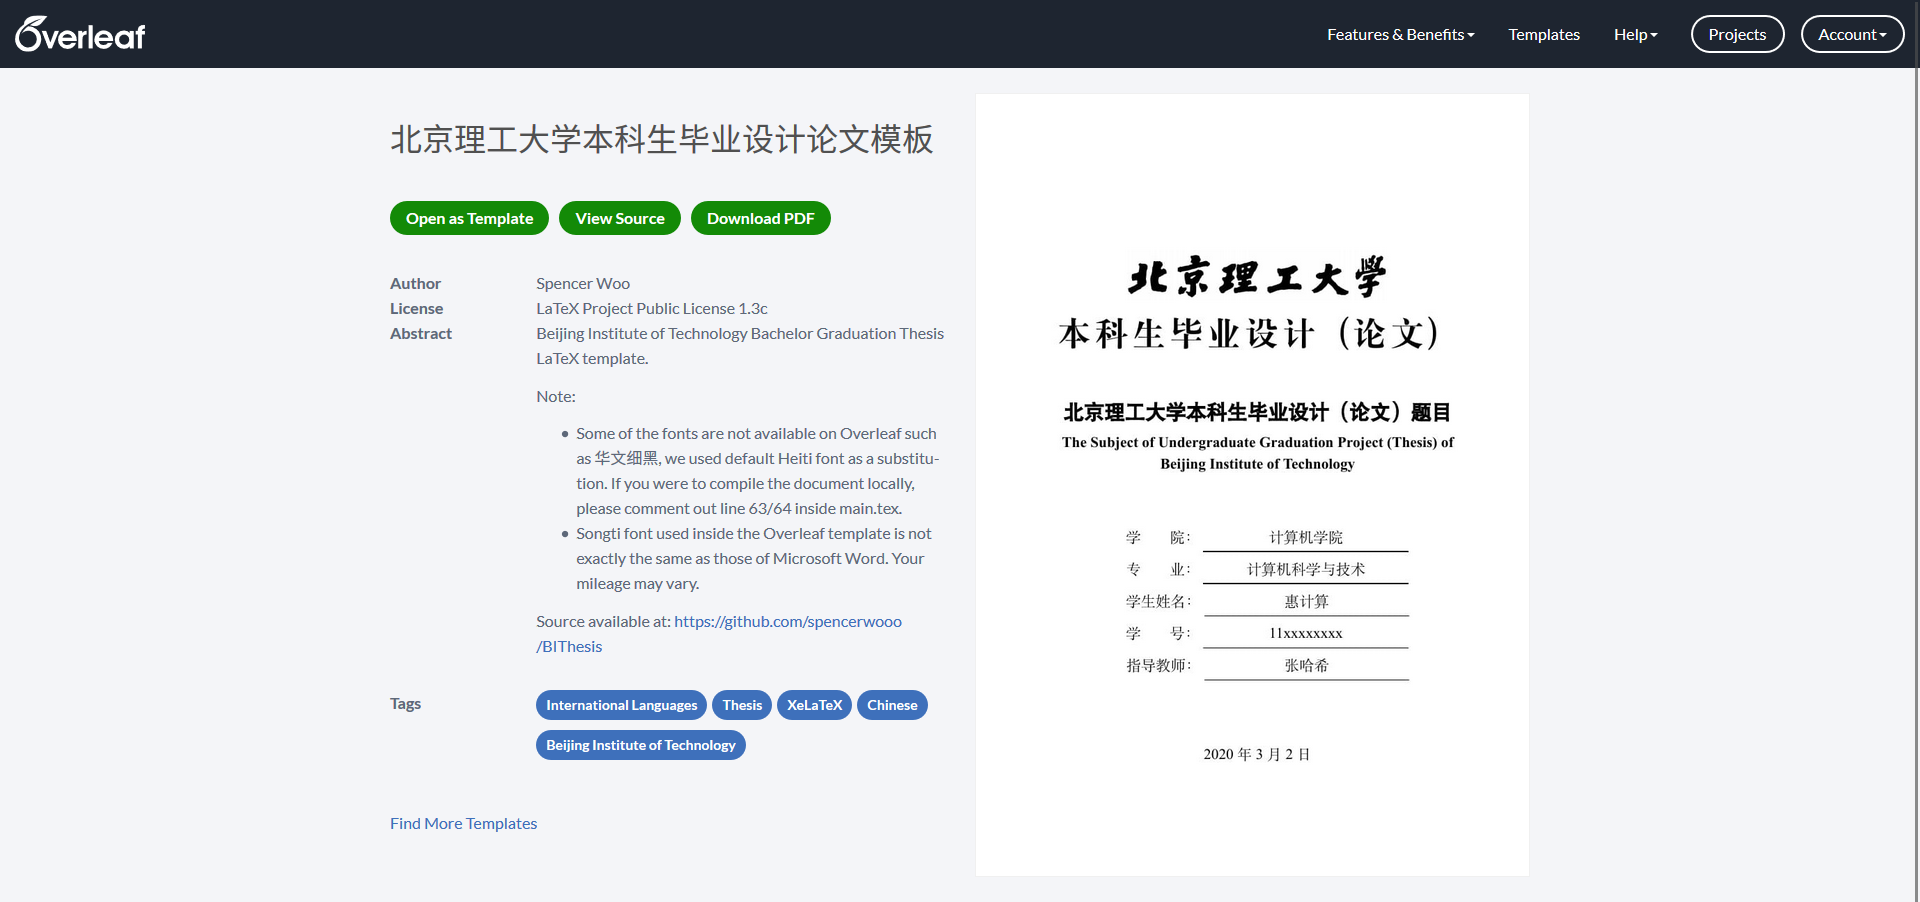
\includegraphics[width=\textwidth]{images/overleaf_grad_thesis.png}
  \caption{Overleaf 在线版本的毕业论文模板}
\end{figure}

Overleaf 版本的毕业论文模板中由于没有微软版权字体“华文细黑”,导致封面的毕业论文中文大标题无法用 Word 模板中规定的字体渲染,使得最终呈现样式与要求有些出入,如果希望保证 {\LaTeX} 模板输出和学校模板一致,那么还是推荐在本地进行撰写和编译。

\subsubsection{在本地撰写}

由于:

\begin{itemize}
  \item {\BIThesis} 文章主体部分是中文,使用了 \texttt{ctex} 宏包,因此需要使用 \texttt{xelatex} 进行全文编译
  \item 参考文献部分使用了 {Bib\LaTeX},因此需要使用 \hologo{biber} 进行参考文献的编译
\end{itemize}

\paragraph{使用 {\hologo{XeLaTeX}} 编译}
整个项目的编译工具链的顺序为:

\begin{center}
  \begin{tikzpicture}[
    bib/.style={rectangle, draw=ForestGreen!60, fill=ForestGreen!5, very thick, minimum size=8mm},
    xe/.style={rectangle, draw=RubineRed!60, fill=RubineRed!5, very thick, minimum size=8mm},
    ]
  % Nodes
  \node[xe] (xelatex1) {xelatex};
  \node[bib] (biber) [right=of xelatex1] {biber};
  \node[xe] (xelatex2) [right=of biber] {xelatex};
  \node[xe] (xelatex3) [right=of xelatex2] {xelatex};

  % Arrows
  \draw[->] (xelatex1.east) -- (biber.west);
  \draw[->] (biber.east) -- (xelatex2.west);
  \draw[->] (xelatex2.east) -- (xelatex3.west);
  \end{tikzpicture}
\end{center}


其中,按照 VS Code 的 LaTeX Workshop 设置格式:

\begin{itemize}
  \item {\hologo{XeLaTeX}} 的编译命令为:
  \begin{minted}[frame=single]{json}
  {
    "name": "xelatex",
    "command": "xelatex",
    "args": [
      "-synctex=1",
      "-interaction=nonstopmode",
      "-file-line-error",
      "-pdf",
      "-outdir=%OUTDIR%",
      "-cd",
      "%DOC%"
    ],
    "env": {}
  }
  \end{minted}
  \item {\hologo{biber}} 的编译命令为:
  \begin{minted}[frame=single]{json}
  {
    "name": "biber",
    "command": "biber",
    "args": [
        "%DOCFILE%"
    ],
    "env": {}
  }
  \end{minted}
\end{itemize}

那么,整个编译的 recipe 即为:

\begin{minted}[frame=single]{json}
  {
    "name": "xelatex -> biber -> xelatex * 2",
    "tools": [
        "xelatex",
        "biber",
        "xelatex",
        "xelatex"
    ]
  }
\end{minted}

\paragraph{使用 latexmk 编译}
如果你使用 \texttt{latexmk},也可以使用如下的编译方法:

\begin{itemize}
  \item \texttt{latexmk} 的编译命令:
  \begin{minted}[frame=single]{json}
  {
    "name": "latexmk",
    "command": "latexmk",
    "args": [
        "-synctex=1",
        "-interaction=nonstopmode",
        "-file-line-error",
        "-xelatex",
        "-outdir=%OUTDIR%",
        "-cd",
        "%DOC%"
    ],
    "env": {}
  }
  \end{minted}
\end{itemize}

那么,整个编译的 recipe 即为:
\begin{minted}[frame=single]{json}
  {
    "name": "latexmk 🔃",
    "tools": [
        "latexmk"
    ]
  }
\end{minted}

\subsection{你的内容从哪里开始?}

\subsubsection{开始}

\subsubsection{中英摘要}

\subsubsection{正文}

\subsubsection{后续模块}

\subsection{参考文献管理}

\subsection{图片素材}

\subsection{表格插入}

\subsection{公式插入}

\subsection{其他}

\subsubsection{代码高亮}

\subsubsection{算法模块}
